\documentclass[reprint, nobibnotes, amssymb, amsmath, amsfonts, physics, mathtools, mathrsfs, floatfix]{revtex4-1}
\usepackage{graphicx}
\usepackage[english]{babel}

\newcommand{\redchi}{$\tilde{\chi}^2\,$}

\newcommand{\moss}{M\"{o}ssbauer }

\begin{document}

  \title{\moss Spectroscopy of Fe-57}

  \author{Aman LaChapelle}
  \affiliation{The University of Chicago}

  \begin{abstract}
    We use \moss spectroscopy to determine several properties of excited Fe-57.  Using Stainless Steel, we measure the linewidth of the excited state of Fe-57 to be XXXXXXX, corresponding to a lifetime of XXXXXXX.  This leads us to an isomer shift of XXXXXXX.  We also use a magnetic Fe-57 sample to measure the Zeeman splitting of nuclear energy levels of XXXXXX, a nuclear magnetic moment of XXXXXXX and the magnetic field at the nucleus of XXXXXXXX.  Finally, we make use of an electric quadrupole sample in order to determine $\tilde{Q}\frac{\partial E}{\partial z} = XXXXXXXXX$ at the sample, and find $\frac{\partial E}{\partial z} = XXXXXXXXX$ at the sample.
  \end{abstract}

  \maketitle
  \tableofcontents

  \section{Introduction and Theory}
    We seek to perform a number of measurements using the technique of \moss spectroscopy.  The principle is that we are able to use doppler shift to measure energies at remarkably tiny scales.  We will achieve incredibly high precision in our measurements by using a fixed source that we move with a known velocity in order to make use of the doppler shift phenomenon to alter the energy of the source by a tiny amount.  We need this high resolution because the phenomena we are measuring take place and induce shifts of the order of $10^{-7}$ eV, and this causes difficulty for many experiments.  Other types of experiments are also able to examine phenomena with resolution like the \moss technique, but are by far more complicated, and furthermore measure different phenomena in general.  Many AMO experiments make use of lasers and sub-MHz resolution to examine similar features of nuclei, but their setups are far more complicated and experiments are much more time-intensive and expensive.  Therefore, in order to measure nuclear phenomena in metallic crystals, we make use of this \moss technique.

    \subsection{Isomer Shift}
      This effect emerges from the embedding of a nucleus in a heterogeneous chemical environment.  In our case we work with Stainless Steel, alloy 302, whose chemical composition is outlined in Table~\ref{tab:SS_chemical_makeup}.  Approximately 70\% of the alloy is Iron, and of that only a tiny percentage (approx. 1\%) is Fe-57.  This is an ideal environement to see the isomer shift because it is enough Fe-57 that we will be able to see a peak develop, but not so much that we have more excited iron than other chemicals and so our isomer shift will be strong and present.  We can determine the energy of the shifted transition with the following:
      \begin{equation}
        \Delta E_{iso} = \delta + \Delta E_0
      \end{equation}
      with $E_0$ being the energy before the shift, $\delta$ being the isomer shift, and $E_{iso}$ being the energy after the shift.  We know that the transition we are looking for has a certain energy, and by fitting the transition dip that we see from our \moss spectrum, we will be able to determine $E_{iso}$.

  \section{Conclusion, Tables and Figures}

    \subsection{Tables}
      \begin{table}[h]
        \centering
        \begin{tabular}{|c|c|}
          \hline
          Element & Content (\%) \\ \hline
          Cr & 17-19 \\ \hline
          Ni & 8-10 \\ \hline
          Mn & 2 \\ \hline
          Si & 1.00 \\ \hline
          C & 0.15 \\ \hline
          S & 0.03 \\ \hline
          P & 0.045 \\ \hline
        \end{tabular}
        \caption{The remainder is Fe, mostly Fe-56.~\cite{stainless_chemical_makeup}~\label{tab:SS_chemical_makeup}}
      \end{table}

      \begin{table}[h]
        \centering
        \begin{tabular}{|c|c|c|}
          \hline
          Quantity & Value & Uncertainty \\ \hline
          $I_0$ ($eV/s/m^2$) & 7.13e+02 & 2.51e+01 \\ \hline
          $\Gamma$ ($eV$) & 2.0e-08 & 1e-09 \\ \hline
          $\delta$ ($eV$) & -1.21e-08 & 3e-10 \\ \hline
          $C$ & 1574 & 3 \\ \hline
        \end{tabular}
        \caption{Fit values for our Stainless Steel spectrum.  The covariance matrix for this fit was well-defined, so the uncertainties on this fit simply come from the diagonals of the covariance matrix.~\label{tab:ss_fit_stats}}
      \end{table}

      \begin{table}[h]
        \centering
        \begin{tabular}{|c|c|c|}
          \hline
           Quantity (indexed by peak) & Value & Uncertainty \\ \hline
           $I_{0, 1}$ ($eV/m^2/s$) & 4.3e+02 & 8e+01 \\ \hline
           $I_{0, 2}$ ($eV/m^2/s$) & 3.9e+02 & 9e+01 \\ \hline
           $I_{0, 3}$ ($eV/m^2/s$) & 2e+02 & 10e+01 \\ \hline
           $I_{0, 4}$ ($eV/m^2/s$) & 2.5e+02 & 7e+01 \\ \hline
           $I_{0, 5}$ ($eV/m^2/s$) & 3.7e+02 & 8e+01 \\ \hline
           $I_{0, 6}$ ($eV/m^2/s$) & 3.8e+02 & 9e+01 \\ \hline
           $\Gamma_1$ ($eV$) & 1.6e-08 & 1e-09 \\ \hline
           $\Gamma_2$ ($eV$) & 1.4e-08 & 2e-09 \\ \hline
           $\Gamma_3$ ($eV$) & 1.3e-08 & 3e-09 \\ \hline
           $\Gamma_4$ ($eV$) & 1.6e-08 & 2e-09 \\ \hline
           $\Gamma_5$ ($eV$) & 1.6e-08 & 3e-09 \\ \hline
           $\Gamma_6$ ($eV$) & 2.0e-08 & 3e-09 \\ \hline
           $\delta_{1}$ ($eV$) & -2.53e-07 & 1.7e-08 \\ \hline
           $\delta_{2}$ ($eV$) & -1.51e-07 & 1.7e-08 \\ \hline
           $\delta_{3}$ ($eV$) & -4.57e-08 & 1.7e-08 \\ \hline
           $\delta_{4}$ ($eV$) & 3.27e-08 & 1.7e-08 \\ \hline
           $\delta_{5}$ ($eV$) & 1.41e-07 & 1.7e-08 \\ \hline
           $\delta_{6}$ ($eV$) & 2.52e-07 & 1.7e-08 \\ \hline
           $C_1$ (counts) & 2.34e+03 & 2e+01 \\ \hline
           $C_2$ (counts) & 2.30e+03 & 2e+01 \\ \hline
           $C_3$ (counts) & 2.300e+03 & 1.4e+01 \\ \hline
           $C_4$ (counts) & 2.30e+03 & 2e+01 \\ \hline
           $C_5$ (counts) & 2.300e+03 & 1.5e+01 \\ \hline
           $C_6$ (counts) & 2.3000e+03 & 1.16e+01 \\ \hline
        \end{tabular}
        \caption{Fit values for Fe-57.  $\delta$ signifies distance from the center, which is set to 14.4 keV.  The covariance matrix was not well-defined so uncertainties were determined by running the fit on randomized points chosen from a normal distribution around each points best-guess value, iterating 300 times, and taking the standard deviation of those values.  The values of C from 2 to 6 are the same because of the way that the fit was performed - there was a bias so that those values would end up the same to reduce the computational intensity of the fitting function.  The uncertainties were different, so we decided to show them all anyway.~\label{tab:fe_57_fit}}
      \end{table}

      \begin{table}[h]
        \begin{tabular}{|c|c|c|}
          \hline
          Quantinty (indexed by peak) & Value & Uncertainty \\ \hline
          $I_{0, 1}$ ($eV/m^2/s$) & 3.26e+02 & 6e+00 \\ \hline
          $I_{0, 2}$ ($eV/m^2/s$)& 3.9e+02 & 2.5e+01 \\ \hline
          $\Gamma_1$ ($eV$) & 1.4e-08 & 2e-09 \\ \hline
          $\Gamma_2$ ($eV$) & 9.85e-09 & 6e-10 \\ \hline
          $\delta_{1}$ ($eV$) & -6.0e-08 & 4e-09 \\ \hline
          $\delta_{2}$ ($eV$) & 2.1e-08 & 4e-09 \\ \hline
          $C_1$ (counts) & 3.0e+03 & 3e+02 \\ \hline
          $C_2$ (counts) & 2.3e+03 & 3e+02 \\ \hline
        \end{tabular}
        \caption{Fit values for the Quadrupole sample.  $\delta$ signifies distance from the center, which is set to 14.4 keV.  Again, the covariance matrix was not well-defined so we used the method of running the fit on randomly chosen data points within the normal distribution centered at each best-guess point.  The standard deviation converged in just under 100 runs for this case, so we used 100 iterations.~\label{tab:quad_fit}}
      \end{table}

    \subsection{Figures}
    \begin{widetext}

      \begin{figure}[h]
        \centering
        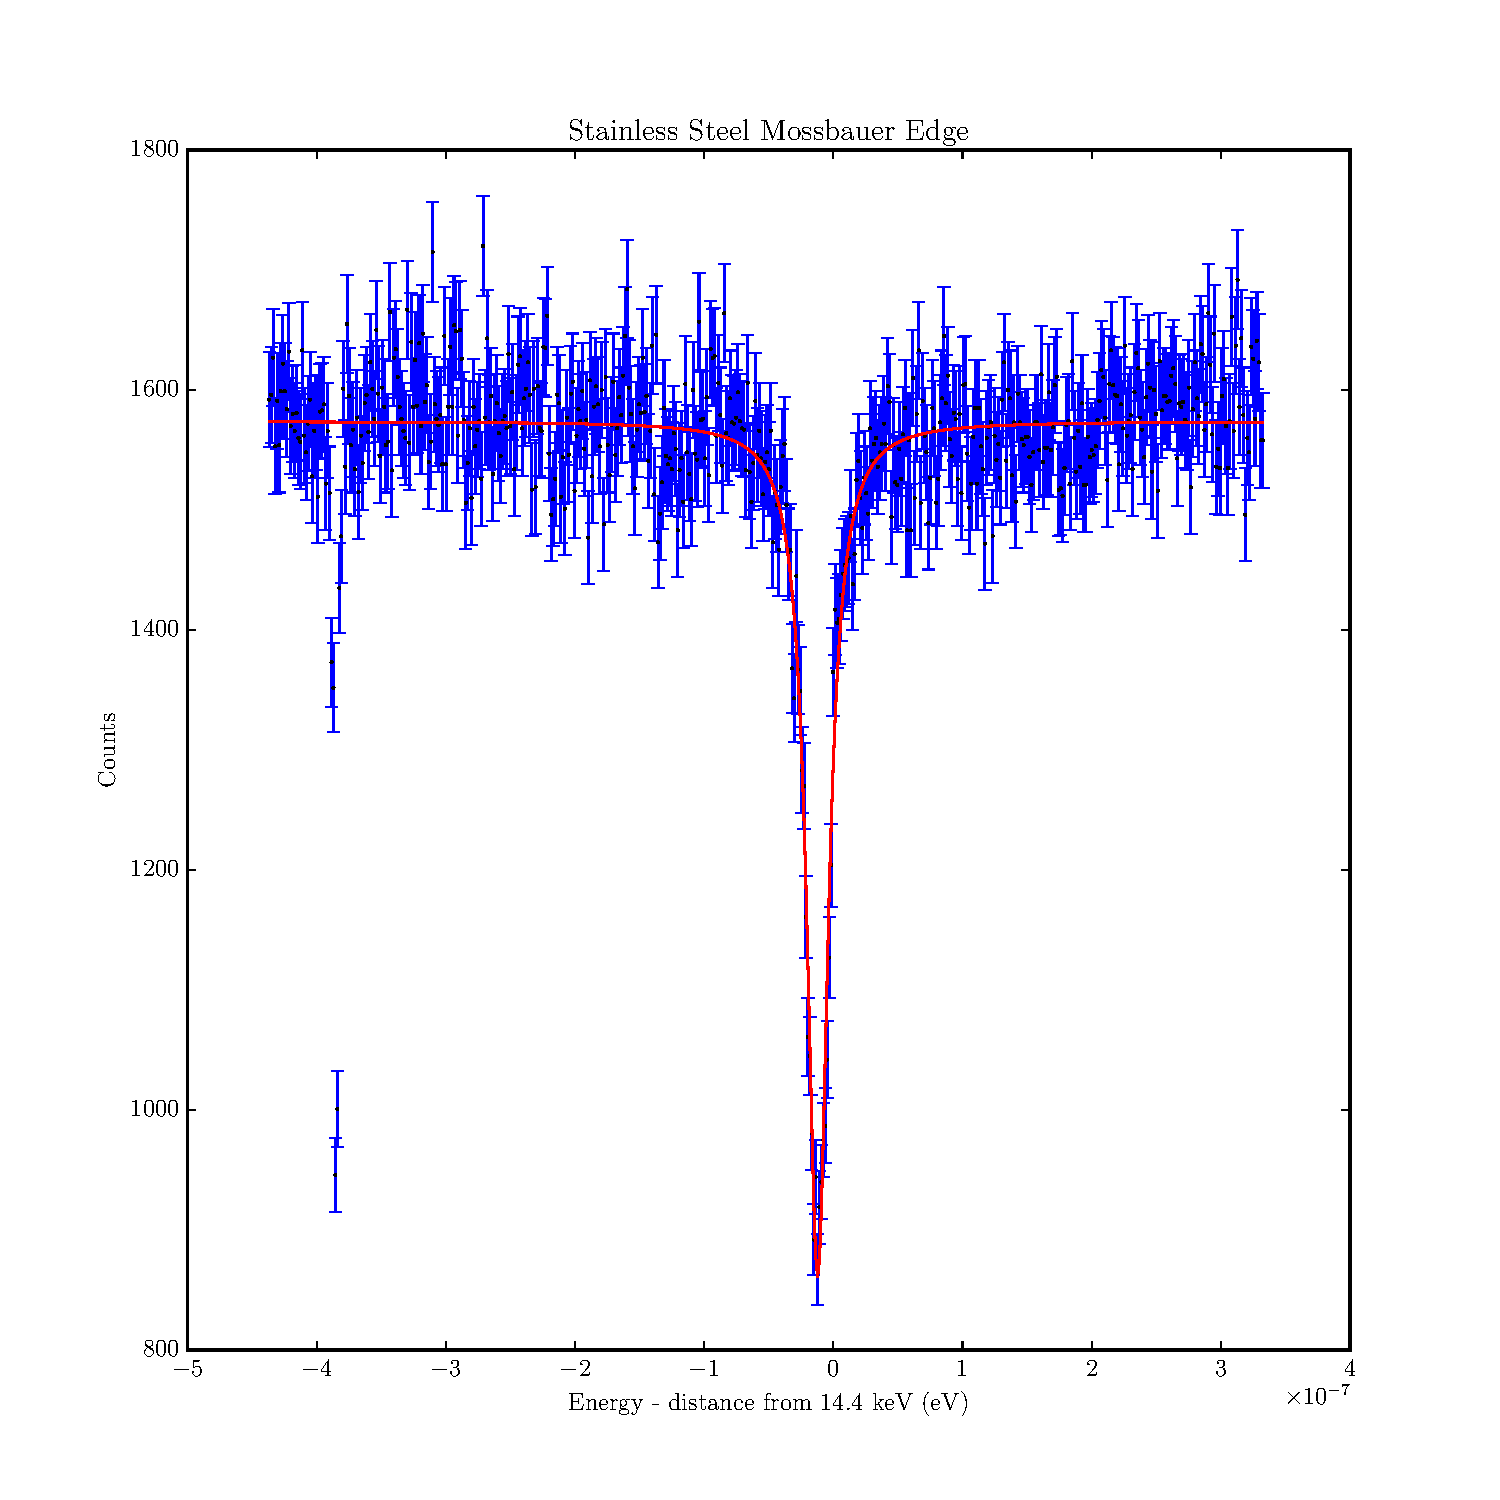
\includegraphics[width=\linewidth]{../plots/ss_fit.pdf}
        \caption{
          Fitting the spectrum for Stainless Steel Grade 302 in order to determine the isomer shift of the Fe-57 contained in the sample.  We fit to the form: \\
            $I(E) = -I_0 \frac{(\Gamma/2)^2}{(E - \delta)^2 + (\Gamma/2)^2}$ \\
          with values held in Table~\ref{tab:ss_fit_stats}.  The \redchi value was a little high, but for a fit with such a large background deviation, we should not be overly worried.  We return for the fit $\tilde{\chi}^2 = 2.09$.  We should note that here and going forward, we use $\delta$ to refer to distance from 0, or in our case, 14.4 keV.  Thus all our values for peak centers are expressed in terms of distance from 14.4 keV.
          ~\label{ss_fit}
        }
      \end{figure}

      \begin{figure}[h]
        \centering
        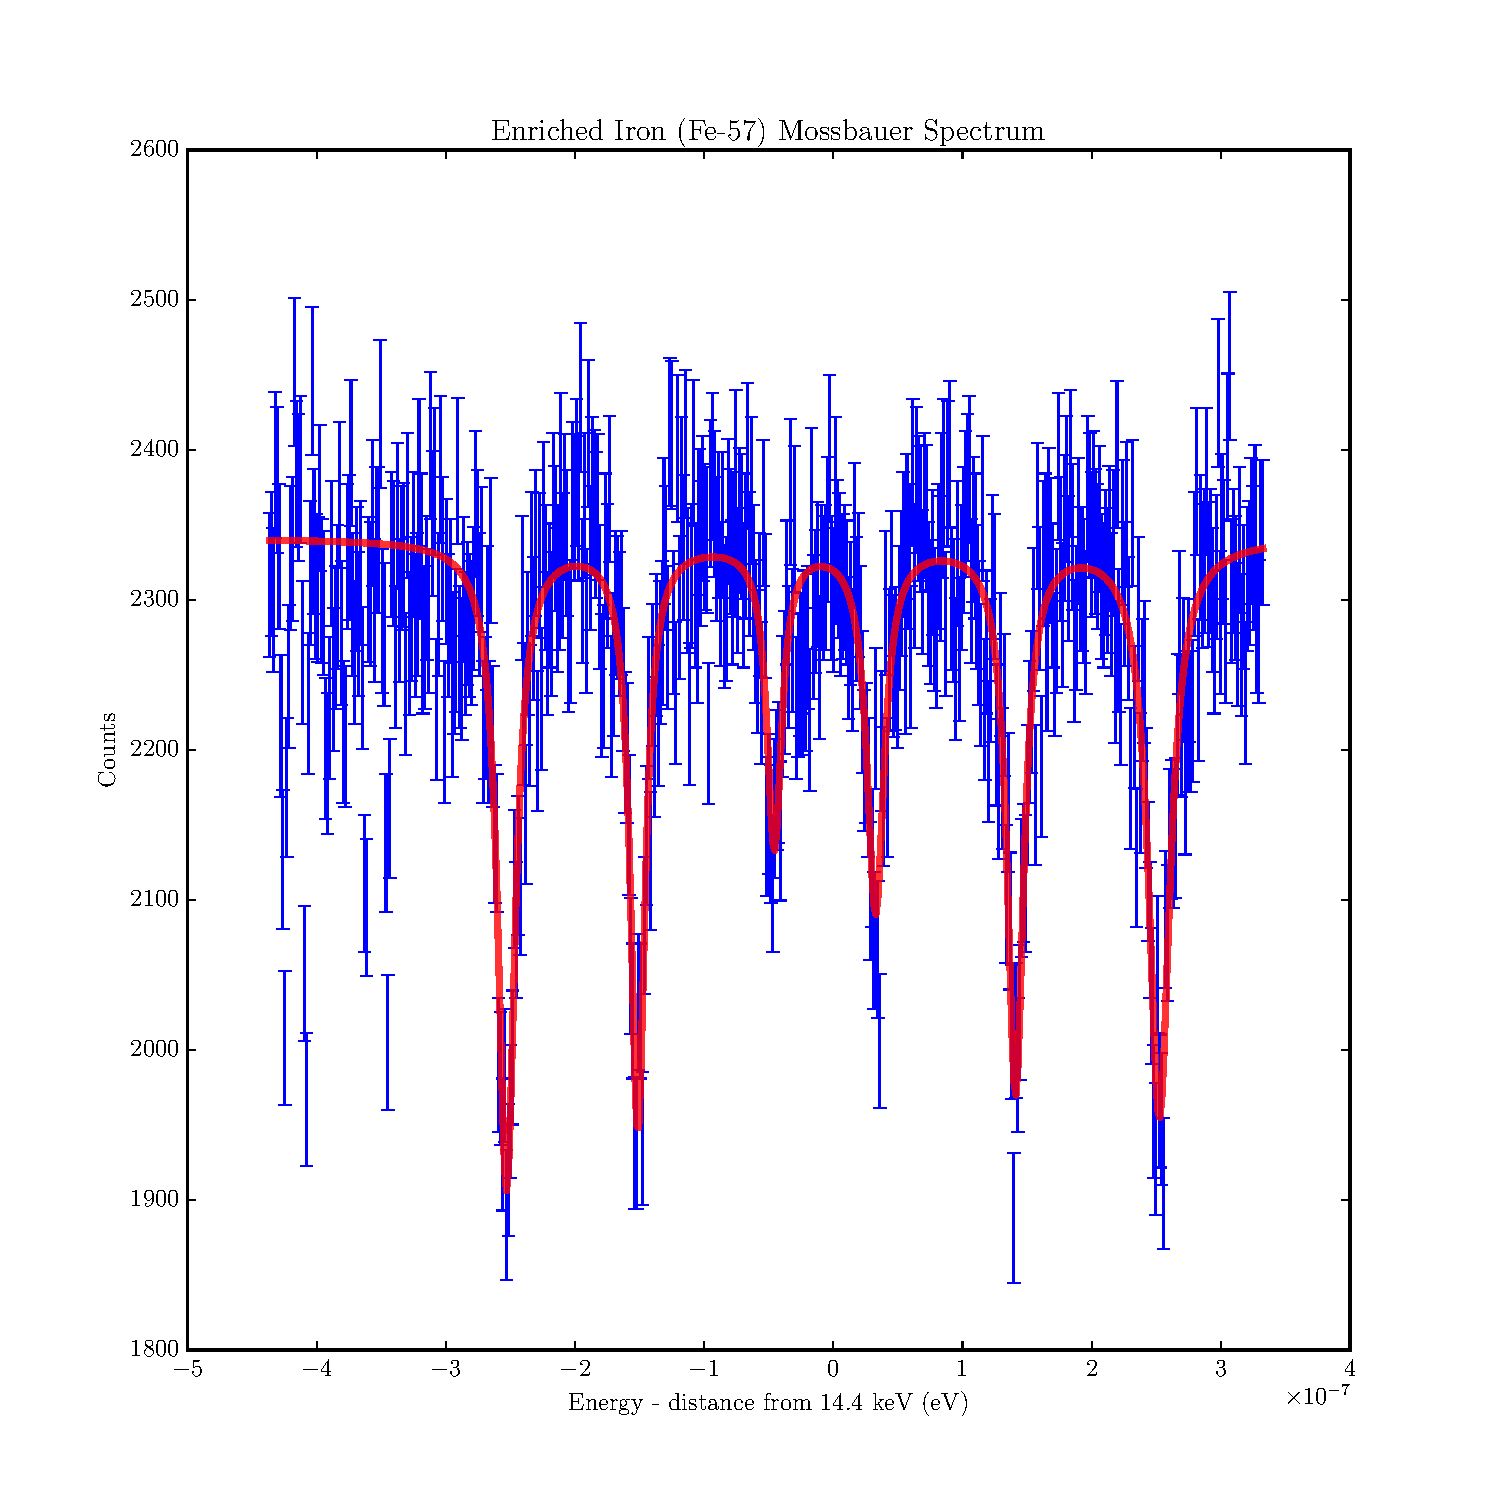
\includegraphics[width=\linewidth]{../plots/fe_fit.pdf}
        \caption{Fitting the spectrum for the Fe-57 sample to determine the Zeeman splitting of the atomic energy levels.  Fit values are held in Table~\ref{tab:fe_57_fit}.  We fit to a function: \\
          $I(E) = C - \sum\limits_{i = 0}^{i = 5}{ \frac{(\Gamma_i/2)^2}{(E-\delta_i)^2 + (\Gamma_i/2)^2} }$ \\
        The \redchi value was an astounding $\tilde{\chi}^2 = 1.71$.  This leads us to believe that the model chosen was indeed correct.~\label{fe_fit}}
      \end{figure}

      \begin{figure}[h]
        \centering
        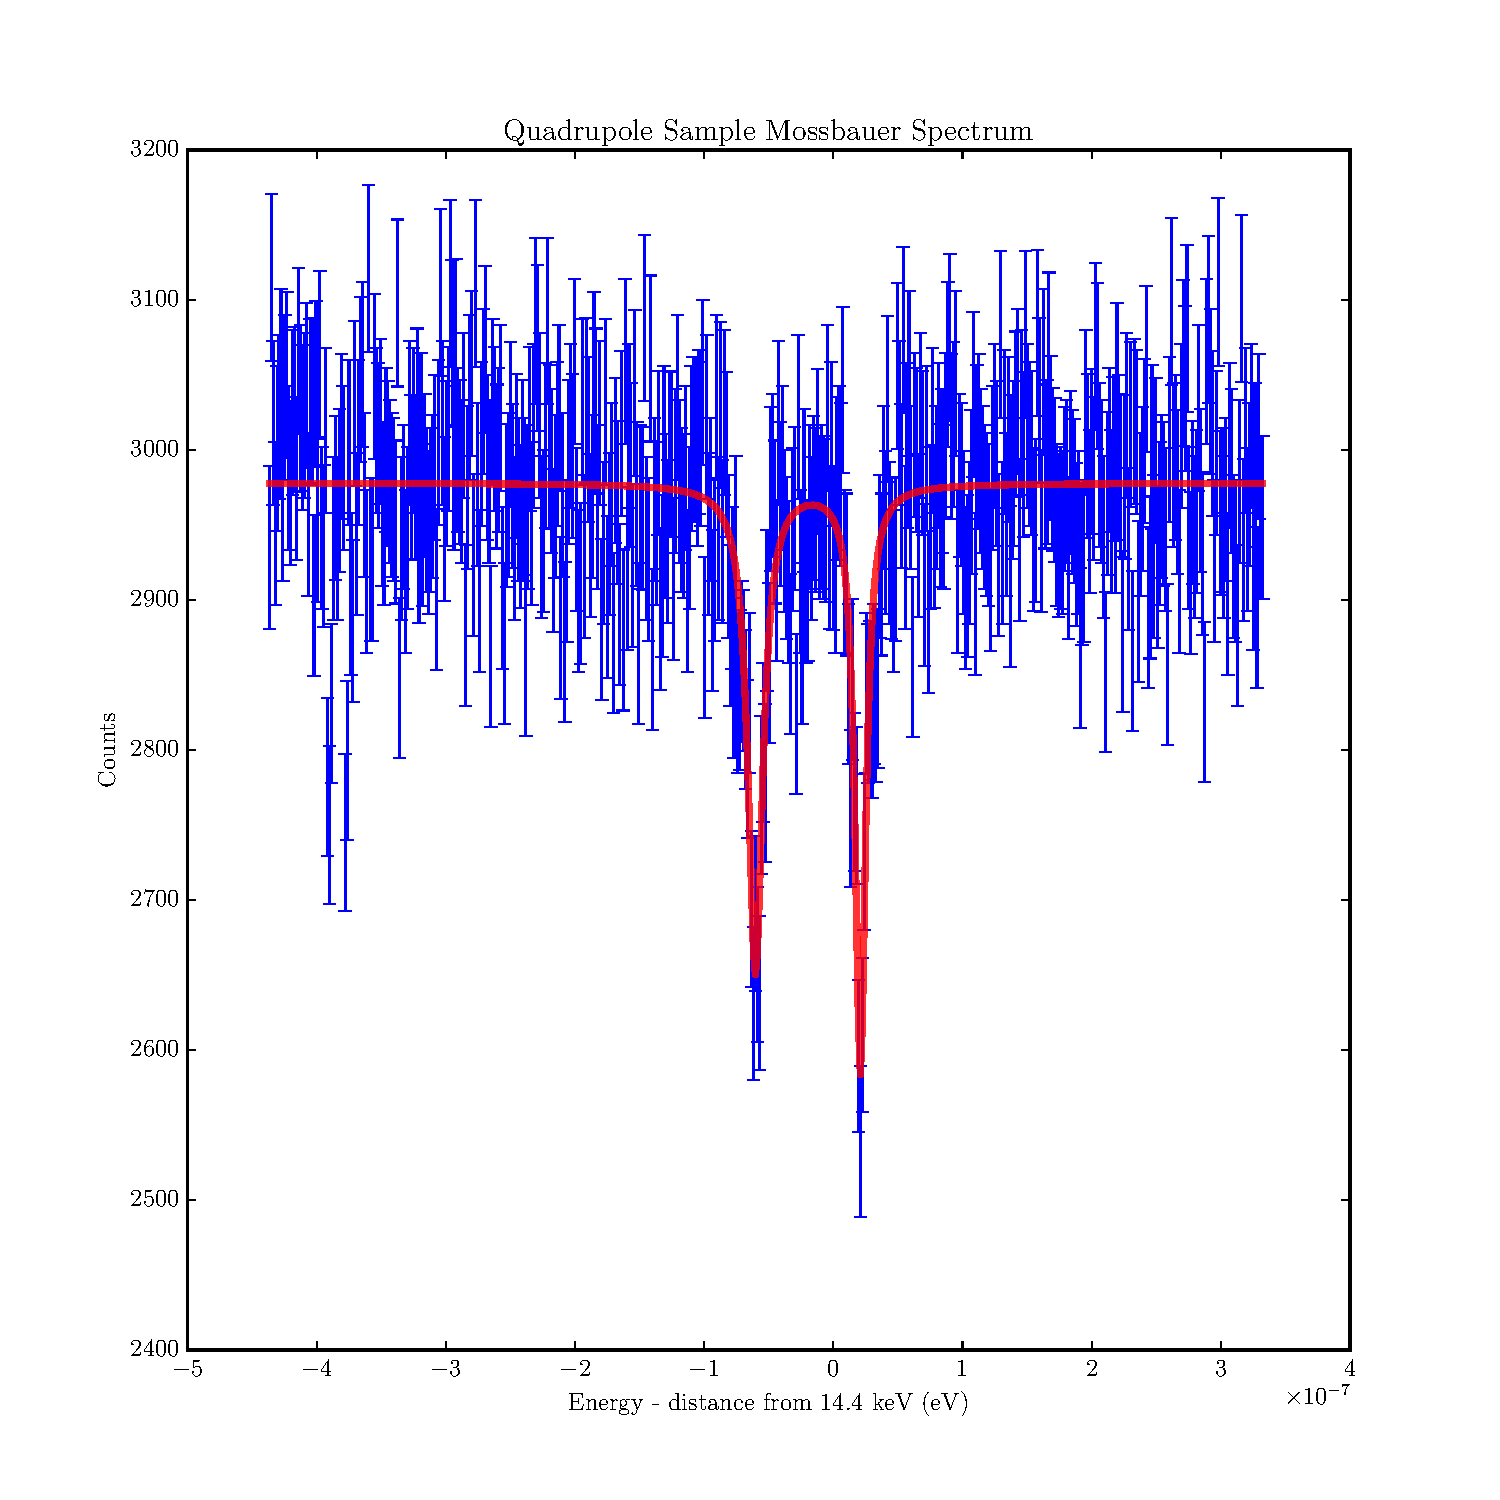
\includegraphics[width=\linewidth]{../plots/quadrupole.pdf}
        \caption{Fitting the spectrum for the Quadrupole sample to determine the quadrupole splitting.  Fit values are held in Table~\ref{tab:quad_fit}.  We fit to a function: \\
          $I(E) = C - \sum\limits_{i = 0}^{i = 1}{ \frac{(\Gamma_i/2)^2}{(E-\delta_i)^2 + (\Gamma_i/2)^2} }$ \\
        The \redchi value was $\tilde{\chi}^2 = 1.07$.~\label{quadrupole_fit}}
      \end{figure}

    \end{widetext}

    \bibliography{bibliography}
    \bibliographystyle{plain}

\end{document}
